\chapter{Symbolic Client Verification}
\label{ch:scv}

%In this chapter we describe how symbolic execution can be used to
%verify that a message sequence is consistent with a sanctioned version
%of the client software. 
%In this chapter, we develop an approach to detect a significant class of
%cheats in which a player changes a game client to allow behaviors that
%a sanctioned game client would not allow.  To accomplish this, the
%player might modify the client executable or in-memory data structures
%of a running client, for example.  Today, the most robust defense
%against such client modification is to maintain authoritative state at
%the server, beyond the reach of direct manipulation by cheaters.  This
%defense, however, exacts a heavy price from game operators, owing to
%the increased bandwidth use that results from sending low-level
%client events (in the limit, every player input) to the server for
%accessing such state and conveying the effects back to clients.  As
%bandwidth is one of the largest costs for large-scale game
%operators~\cite{mulligan03:guide} and also a recurring one, this
%tension between bandwidth use and cheat prevention is problematic:
%\begin{quote}
%{\sl In the US and European markets, a good goal to shoot for is 4-6
%kilobits per second (kps)/player or less. ... If you can get the bit
%rate down to 2kps, you're ``golden.''  It's hard to see how that can
%happen, however, without putting dangerous amounts of data directly
%into the client, which is just asking for trouble from talented
%cheaters and hackers.}~\cite[p.~112]{mulligan03:guide}
%\end{quote}
%The movement of games to all manners of devices using wireless,
%volume-priced communication only reinforces the importance
%of keeping bandwidth utilization to a minimum.  Moreover, even with
%the amount of detailed client information collected at the server,
%server-side checking today is heuristic (and thus potentially
%incomplete) and manually programmed (and thus effort-intensive):
%\begin{quote}
%{\sl Players love to cheat --- especially in online games ... be
%ready to add server-side support to prevent user cheating with
%methods that you were not able to predict.}~\cite{hawkins03:quote}
%\end{quote}

In this chapter we demonstrate a technique to detect any type of
client modification that causes the client to exhibit behavior, as
seen by the server, that is inconsistent with the sanctioned client
software and the game state known at the server.  That is, our
approach discerns whether there was {\em any possible sequence} of
user inputs to the sanctioned client software that could have given
rise to each message received at the server, given what the server
knew about the game client based on previous messages from the client
and the messages the server sent to the client. In doing so, our
approach remedies the previously heuristic and manual construction of
server-side checks. Moreover, our approach potentially enables new
client designs that reduce bandwidth use by placing more authoritative
state at the client, since our approach verifies that the client's
behavior is consistent with legal management of that state.  While
reducing interaction with the client will generally increase the
computational cost of our verification, verification need not be done
on the critical path and can be performed selectively (e.g., only for
randomly selected or suspicious users).  
%Moreover, it can benefit from
%the dramatic growth of inexpensive computing power (larger numbers of
%cores) in game-operator server farms.

Our strategy exploits the fact that clients are often structured
as an event loop that processes user inputs, server messages, or other
events in the context of current client state and then sends an update
to the server on the basis of its processing.  We symbolically execute
the loop to derive a predicate that characterizes the effects of the
loop, and specifically the update sent to the server, as a function of
its inputs and game state.  By partially instantiating these
predicates on the basis of the actual messages the server receives
from a client and what the server previously sent to the client, a
{\em \verifier} can then use a constraint solver to determine whether
the resulting predicate is satisfiable.  If so, then the messages are
consistent with proper client execution --- i.e., there were {\em
  some} user inputs that could have yielded these messages.

We demonstrate our approach with three case studies on online games.
First, we apply our technique to the open-source game \xpilot. Because
\xpilot was developed as is commonplace today, i.e., with low-level
client events being sent to the server, this case study does not fully
illustrate the strengths of our approach.  However, it does
demonstrate the (few) ways in which we found it necessary to adapt
\xpilot to use our technique efficiently.  For the second case study,
we use a game of our own design that is similar to \pacman but that
has features to better exercise our technique.  Third, we utilize
\tetrinet, a multiplayer version of \tetris, to demonstrate the
potential bandwidth savings that symbolic client verification can
enable.  
Together, these case studies illustrate the limits and
benefits of our approach and serve as a foundation for future work.
%and serve as guidance for game developers who
%wish to use this technique for detecting cheating in their games.

Following our initial investigation of these case studies, we
investigate the impact of message loss on our verification technique.
We extend our technique to improve verification performance in the
face of message loss on the network.  We then evaluate this extension
using \xpilot, since it is an example of a game built to use an
unreliable transport protocol for performance reasons and consequently
to continue operation despite message loss.

\section{Goals, Assumptions and Limitations}
\label{sec:scv:background}

\ignore{
The defense that we develop in this chapter addresses a class of game
cheats that Webb and Soh term {\em Invalid commands}:
\begin{quote}
{\sl Usually implemented by modifying the game client, the invalid
command cheat results in the cheater sending commands that are not
possible with an unmodified game client. Examples include giving the
cheater's avatar great strength or speed. This may also be implemented
by modifying the game executable or data files. Many games suffer this
form of cheating, including console games such as
\gearsofwar.}~\cite[Section 4.2.3]{webb08:survey}
\end{quote}
Importantly, our technique will even detect commands that are invalid
in light of the history of the client's previous behaviors witnessed
by the server, even if those commands could have been valid in
some other execution.  Simply put, our approach will detect any client
message sequence that is impossible to observe from the sanctioned client
software.
}
Importantly, our technique will even detect commands that are invalid
in light of the history of the client's previous behaviors witnessed
by the server, even if those commands could have been valid in
some other execution.  Simply put, our approach will detect any client
message sequence that is impossible to observe from the sanctioned client
software.

%We designed our cheat detection technique primarily for use by game developers. 
As we present and evaluate our approach, it requires
access to source code for the client, though potentially a similar
approach could be developed with access to only the executable.
The approach should be attractive to developers because it can
save them significant effort in implementing customized server-side
verification of client behaviors.  Our approach is comprehensive and
largely automatic; in our case study described in \secref{sec:scv:xpilot},
we needed only modest adaptations to an existing open-source game.

In order for detection to be efficient, our technique depends on
certain assumptions about the structure of the client.  We assume
in this dissertation that the client is structured as a loop that
processes inputs (user inputs, or messages from the server) and
that updates the server about certain aspects of its status that
are necessary (e.g., the client's current
location on a game map, so that the server can update other players in
the game with that location).  Updates from the client to the server
need not be in exact one-to-one correspondence to loop iterations.
However, as the number of loop iterations that execute without sending
updates increases, the uncertainty in the \verifier's ``model'' of the
client state also generally increases.  This increase will induce
greater server-side computation in verifying that future updates from
the client are consistent with past ones.  As we will see in
\secref{sec:scv:xpilot}, it is useful for these updates from the client to
indicate which server-to-client messages the client has received, but
importantly, the information sent by the client need not include the
user inputs or a full account of its relevant state.  Indeed, it is
this information that a client would typically send today and
that we permit the client to omit in our approach.

Due to the scope of what it tries to detect, however, our technique
has some limitations that are immediately evident.  First, our
technique will not detect cheats that are permitted by the sanctioned
client software due to bugs.  Second, modifications to the client
that do not change its behavior as seen at the server will go
unnoticed by our technique.  For example, any action that is possible
to perform will be accepted, and so cheating by
modifying the client program to make difficult (but possible) actions
easy will go undetected.  Put in a more positive light, however, this
means that our technique has no false alarms, assuming that symbolic
execution successfully explores all paths through the client.  As
another example, a client modification that discloses information to
the player that should be hidden, e.g., such as a common cheat that
uncovers parts of the game map that should be obscured, will go
unnoticed by our technique.  In the limit, a user could write their 
own version of the client from scratch and still go undetected,
provided that the behaviors it emits, as witnessed by the server, are
a subset of those that the sanctioned client software could emit.

\section{Client Verification Approach}
\label{sec:scv:exhaustive}
\label{sec:scv:approach}

Our detection mechanism analyzes client output (as seen by the
server) and determines whether that output could in fact have been
produced by a valid client.  Toward that end, a key step of our
approach is to profile the client's source code using symbolic
execution and then use the results in our analysis of observed client
outputs.  
We begin with an application of symbolic execution; shown in our context in
\secref{ssec:scv:approach:constraint}--\secref{ssec:scv:approach:messages}.
The symbolic execution engine that we use in our work is
\klee~\cite{cadar08:klee}, with some modifications to make it more
suitable for our task.

Before we continue, we clarify our use of certain terminology.  Below,
when we refer to a {\em valid} client, we mean a client that
faithfully executes a sanctioned client program (and does not
interfere with its behavior).  Values or messages are then valid if
they could have been emitted by a valid client.

\ignore{
\section{Symbolic Execution}
\label{ssec:scv:approach:symbolic_execution}

Symbolic execution is a way of ``executing'' a program while exploring
all execution paths, for example to find bugs in the program.
Symbolic execution works by executing the software with its initial
inputs specially marked so they are allowed to be ``anything'' --- the
memory regions of the input are marked as symbolic and are not given
any initial value.  The program is executed step-by-step, building
constraints on the symbolic variables based on the program's
operations on those variables.  For example, if the program sets
$\symbexsum \gets \symbexadda+\symbexaddb$, where \symbexsum,
\symbexadda, and \symbexaddb are all marked as symbolic, then after
the operation, there will be a new logical constraint on the value of
\symbexsum that states that it must equal the sum of \symbexadda and
\symbexaddb.  When the program conditionally branches on a symbolic
value, execution forks and both program branches are followed, with
the true branch forming a constraint that the symbolic value evaluates
to true and the false branch forming the opposite constraint.  Using
this strategy, symbolic execution attempts to follow each possible
code path in the target program, building a constraint that must hold
on execution of that path.

Symbolic execution can help locate software bugs by providing
constraints that enable a constraint solver (\klee uses
\stp~\cite{ganesh07:stp}) to generate concrete
inputs that cause errors to occur.  For example, if execution reaches
an error condition (or a state thought to be ``impossible''),
then a constraint solver can use the constraints associated with that
path to solve for a concrete input value which triggers the error
condition.  Having a concrete input that reliably reproduces
an error is a great help when trying to correct the bug in the source
code.
}

At a high level, the symbolic client verification
technique works by generating postconditions for
all of the paths through key event loops in the client application,
and then during verification, constructing chains of postconditions in
combination with the message trace we are verifying. If the complete
postcondition chain is satisfiable, then the message trace could have
been produced by a legitimate client. The computational expense
required for this method of verification lends it to be useful
primarily in an offline fashion and only after modifying test
applications to constrain the search spaces they present.

\subsection{Generating Round Constraints}
\label{ssec:scv:approach:constraint}

The first step of our technique is identifying the main event loop of
the game client and all of its associated client state, which should
include any global memory, memory that is a function of the client
input, and memory that holds data received from the network.  These
state variables are then provided to the symbolic execution tool,
which is used to generate a constraint for each path through the loop
in a single round. These constraints are thus referred to as {\em \pathsegcons}.
\Pathsegcons consist of three classes of symbolic variables: {\em
state} variables, {\em input} variables and {\em network} variables.

\subsubsection{Toy Example}

For example, consider the toy game client in
Figure~\ref{fig:toy:original}.  This client reads a keystroke from the
user and either increments or decrements the value of the location
variable \toyloc based on this key.  The new location
value is then sent to the server, and the client loops to read a new
key from the user.  Although this example is a toy, one can imagine it
forming the basis for a \pong client.

To prepare for symbolic execution, we modify the program slightly, as
shown in Figure~\ref{fig:toy:symbolic}.  First, we initialize the
variable \toykey not with a concrete input value read from the user
(line~\ref{fig:toy:original:keyread}) but instead as an unconstrained
symbolic variable (line~\ref{fig:toy:symbolic:keyread}).  We then
replace the instruction to send output to the server
(line~\ref{fig:toy:original:send}) with a breakpoint in the symbolic
execution (line~\ref{fig:toy:symbolic:break}).  Finally, we create a
new symbolic state variable, \toyoldloc
(line~\ref{fig:toy:symbolic:oldlocinit}), which will represent the
game state up to this point in the execution.  The state variable
\toyloc will be initialized to this previous state
(line~\ref{fig:toy:symbolic:locinit}).  


\begin{figure}[t]
\begin{tabular}[t]{@{\hspace{-0.5em}}c@{\extracolsep{-0.5em}}c}
\subfigure[][{\parbox[t]{0.4\columnwidth}{Toy game client}}]{\label{fig:toy:original}
\begin{minipage}[t]{0.5\columnwidth}
{\footnotesize
\begin{algorithmic}[1]
  \State $\toyloc \gets 0;$ \label{fig:toy:original:locinit}
  \State
  \While{true}
     \State $\toykey \gets \toyreadkey();$ \label{fig:toy:original:keyread}
     \If{$\toykey = \toyesc$}
       \State $\toyendgame();$
     \ElsIf{$\toykey = \toyup$}
        \State $\toyloc \gets \toyloc+1;$
     \ElsIf{$\toykey = \toydown$}
       \State $\toyloc \gets \toyloc-1;$
     \EndIf
     \State $\toysend(\toyloc);$ \label{fig:toy:original:send}
  \EndWhile
\end{algorithmic}
}\vspace{10pt}\end{minipage}
}
&
\subfigure[][{\parbox[t]{0.4\columnwidth}{Symbolically instrumented toy game client}}]{\label{fig:toy:symbolic}
\begin{minipage}[t]{0.5\columnwidth}
{\footnotesize
\begin{algorithmic}[1]
  \State $\toyoldloc \gets \toysymvar;$ \label{fig:toy:symbolic:oldlocinit}
  \State $\toyloc \gets \toyoldloc;$ \label{fig:toy:symbolic:locinit}
  \While{true}
     \State $\toykey \gets \toysymvar;$ \label{fig:toy:symbolic:keyread}
     \If{$\toykey = \toyesc$}
       \State $\toyendgame();$
     \ElsIf{$\toykey = \toyup$}
        \State $\toyloc \gets \toyloc+1;$
     \ElsIf{$\toykey = \toydown$}
       \State $\toyloc \gets \toyloc-1;$
     \EndIf
     \State $\toyMsg \gets \toyloc$
     \State $\toybreak;$ \label{fig:toy:symbolic:break}
  \EndWhile
\end{algorithmic}
}\vspace{10pt}\end{minipage}
}
\end{tabular}
\caption{Example game client}
\label{fig:toy}
\end{figure}

Symbolically executing one loop iteration of this modified program, we
see that there are four possible paths that the client could take in
any given round.  In the first possible path, \toykey is \toyesc, and
the game ends.  Note that this branch never reaches the \toybreak.
The second and third possible paths are taken when \toykey is equal to
\toyup and \toydown, respectively.  The final path is taken when
\toykey is none of the aforementioned keys.  These last three paths
all terminate at the \toybreak.

Via symbolic execution, the \verifier can obtain the constraints for all
symbolic variables at the time each path reached the \toybreak.
Because we artificially created \toyoldloc during the instrumentation
phase, it remains an unconstrained symbolic variable in all three
cases.  The state variable \toyloc, however, is constrained
differently on each of the three paths.  In the case when \toykey is
equal to \toyup, symbolic execution reports $\toyloc = \toyoldloc+1$
as the only constraint on \toyloc.  When \toykey is equal to \toydown,
the constraint is that $\toyloc = \toyoldloc-1$.  And when \toykey is
not \toyup, \toydown, or \toyesc, the constraint is that $\toyloc =
\toyoldloc$.

Therefore, there are three possible paths that can lead to a
message being sent to the server.  If the server receives a message
from a client --- and the client is a valid client --- then the client
must have taken one of these three paths.  Since each path
introduces a constraint on the value of \toyloc as a function of its
previous value, the \verifier can take the disjunction of these
constraints, along with the current and previous values of \toyloc
(which the server already knows) and see if they are all logically
consistent.  That is, the \verifier can check to see if the change in
values for \toyloc match up to a possible path that a valid game
client might have taken.  If so, then this client is behaving
according to the rules of a valid game client.  The disjunction of
\pathsegcons in this case is:
\begin{equation}
(\toyloc = \toyoldloc+1) \vee (\toyloc = \toyoldloc-1) \vee 
(\toyloc = \toyoldloc)
\label{eqn:toyconstraints}
\end{equation}

For example, suppose the \verifier knows that the client reported
on its previous turn that its \toyloc was 8.  If the client were to
then report its new location as $\toyloc=9$, the \verifier could
simply check to see if the following is satisfiable:
\begin{align*}
& (\toyoldloc = 8) \wedge (\toyloc = 9)~\wedge \\
& [(\toyloc = \toyoldloc+1) \vee (\toyloc = \toyoldloc-1) \vee
   (\toyloc = \toyoldloc)]
\end{align*}
\noindent Of course, it is satisfiable, meaning that the new value
$\toyloc=9$ could in fact have been generated by a valid game client.
Suppose, though, that in the next turn, the client reports his new
position at $\toyloc=12$.  Following the same algorithm, the \verifier
would check the satisfiability of
\begin{align*}
& (\toyoldloc = 9) \wedge (\toyloc = 12)~\wedge \\
& [(\toyloc = \toyoldloc+1) \vee (\toyloc = \toyoldloc-1) \vee
   (\toyloc = \toyoldloc) ]
\end{align*}
Because these \pathsegcons are {\em not} satisfiable, no valid game
client could have produced the message $\toyloc=12$ (in this context).
Therefore, the \verifier can safely conclude that the sender of that
message is running an incompatible game client --- is cheating.

There are also constraints associated with the variable \toykey.  We
have omitted these here for clarity, showing only the constraints on
\toyloc.  We have also omitted the constraints generated by the
preamble of the loop, which in this case are trivial (``$\toyloc =
0$'') but in general would be obtained by applying symbolic execution
to the preamble separately.  Had there been any random coin flips or
reading of the current time, the variables storing the results would
also have been declared symbolic, and constraints generated
accordingly.  While file input (e.g., configuration files) could also be
declared symbolic, in this disseration we generally assume that such input
files are known to the \verifier (e.g., if necessary, sent to the
server at the beginning of game play) and so treat these as concrete.

\ignore{
In summary, the key steps in the process to generate \pathsegcons are as follows:
\begin{enumerate}
  \item {\bf Annotate client state:}
    All memory locations that hold client state should be labelled as
    symbolic. Our algorithm requires that all client state variables
    are allocated by the start of the main event loop. 
  \item {\bf Instrument input sources:} Sources of input to the
    client such as random numbers, time or user input from
    key presses should be symbolically modelled. For example, a call
    to \posixGetCh to read a key pressed by a user should be either
    instrumented or replaced to return a symbolic value, rather than
    an concrete key value.
  \item {\bf Instrument network instructions:} The locations
    in the client where there are calls to the network I/O
    instructions (\sendInstr and \recvInstr
    \footnote{In this dissertation, we abbreviate call instructions to
POSIX \posixSelect, \posixSend and \posixRecv system calls (or their
functional equivalents) with the labels \selInstr, \sendInstr and
\recvInstr.  Our techniques apply to software written to other
interfaces, of course, but would require some of our definitions to be
adapted accordingly.}).
    These calls should also be symbolically modelled. The inputs to a
    network send call are set to be a symbolic buffer.
\end{enumerate}
}


\subsection{Accumulating Constraints}
\label{ssec:scv:approach:tracking}

While the branches taken by a client in each round may not be visible
to the \verifier, the \verifier can keep a set of constraints that
represent possible client executions so far.  Specifically, the
\verifier forms a conjunction of \pathsegcons that represents a
sequence of possible paths through the client's loop taken over
multiple rounds; we call this conjunction an {\em \execpathcon } and
denote the set of satisfiable \execpathcons at the end of round
$\roundidx$ by $\execPathConstraints_{\roundidx}$. This set
corresponds to the possible paths taken by a client through round
$\roundidx$.

The \verifier updates a given set $\execPathConstraints_{\roundidx-1}$
of \execpathcons upon receiving a new client message
$\clientMsg_{\roundidx}$ in round $\roundidx$.  To do so, the
\verifier first combines the values given in $\clientMsg_{\roundidx}$
with each \pathsegcon for round \roundidx, where each symbolic
variable in the \pathsegcon represents client state for round
\roundidx, and the \pathsegcon characterizes those variables as a
function of the variables for round $\roundidx-1$.  The verifier then
combines each result with each \execpathcon in
$\execPathConstraints_{\roundidx-1}$ and checks for satisfiability.

For example, let us parameterize the \pathsegcons for the toy example
in \secref{ssec:scv:approach:constraint} with the round number
\genidx:
\[
\genericPathConstraints(\genidx) =
\{~\toyloc_\genidx = \toyloc_{\genidx-1} + 1~,~
   \toyloc_\genidx = \toyloc_{\genidx-1} - 1~,~
   \toyloc_\genidx = \toyloc_{\genidx-1}~\}
\]
\noindent
Note that each member of $\genericPathConstraints(\genidx)$
corresponds to a disjunct in \eqref{eqn:toyconstraints}.  If in round
$\roundidx = 2$ the server receives the message $\clientMsg_2 = 9$
from the client, then it generates the constraint $\msgConstraint =
\mbox{``$\toyloc_2 = 9$''}$, because the value ``$9$'' in the message
represents information corresponding to the variable \toyloc in the
client code.  Then, combining $\msgConstraint$ with each
$\genericPathConstraint \in \genericPathConstraints(2)$ gives the
three constraints:
\[\begin{array}{l}
\toyloc_2 = 9 \wedge \toyloc_2 = \toyloc_1+1\\
\toyloc_2 = 9 \wedge \toyloc_2 = \toyloc_1-1\\
\toyloc_2 = 9 \wedge \toyloc_2 = \toyloc_1
\end{array}
\]
Note that the combination of the client message with each 
\pathsegcon involves both instantiation
(e.g., using $\genidx=2$ above) as well as including the specific
values given in the client message at that round (i.e., $\toyloc_2 =
9$ above).

\begin{figure}[t]
\centering
%\begin{minipage}{0.5\textwidth}
\begin{minipage}{\textwidth}
\begin{algorithm}[H] % must use H inside minipage
  \caption{Symbolic Client Verification}
\begin{algorithmic}[1]
  \Procedure{verify}{$\clientMsg_{\roundidx}$, $\execPathConstraints_{\roundidx-1}$}
  \State $\execPathConstraints_{\roundidx} \gets \emptyset$
  \State $\msgConstraint \gets \msgToConstraint(\clientMsg_{\roundidx})$ \label{fig:trackConstraints:msgConstraint}
  \For{$\genericPathConstraint \in \genericPathConstraints(\roundidx)$}
     \For{$\execPathConstraint \in \execPathConstraints_{\roundidx-1}$}
        \State $\newExecPathConstraint \gets \execPathConstraint \wedge \genericPathConstraint \wedge \msgConstraint$ \label{fig:trackConstraints:newConst}
        \If{$\isSatisfiable(\newExecPathConstraint)$} \label{fig:trackConstraints:isSat}
           \State $\execPathConstraints_{\roundidx} \gets \execPathConstraints_{\roundidx} \cup \{\newExecPathConstraint\}$ \label{fig:trackConstraints:accumulate}
        \EndIf
     \EndFor
  \EndFor
  \EndProcedure
\end{algorithmic}
\end{algorithm}
\end{minipage}
\caption{Construction of $\execPathConstraints_{\roundidx}$ from $\execPathConstraints_{\roundidx-1}$ and $\clientMsg_{\roundidx}$}
\label{fig:trackConstraints}
\end{figure}

These three \pathsegcons each represent a possible path the client
might have taken in the second round.  The \verifier must therefore
consider each of them in turn as if it were the correct path.  For
example, if $\execPathConstraints_1 = \{\toyloc_1 = 8\}$, then the
\verifier can use each \pathsegcon to generate the following possible
\execpathcons:
\[\begin{array}{l}
\toyloc_1 = 8 \wedge [\toyloc_2 = 9 \wedge \toyloc_2 = \toyloc_1+1]\\
\toyloc_1 = 8 \wedge [\toyloc_2 = 9 \wedge \toyloc_2 = \toyloc_1-1]\\
\toyloc_1 = 8 \wedge [\toyloc_2 = 9 \wedge \toyloc_2 = \toyloc_1]
\end{array}
\]

Since the second and third constraints are not satisfiable, however,
this reduces to
\begin{eqnarray*}
\execPathConstraints_2 
& = & \{\toyloc_1 = 8 \wedge [\toyloc_2 = 9 \wedge \toyloc_2 = \toyloc_1+1]\} \\
& = & \{\toyloc_1 = 8 \wedge \toyloc_2 = 9\}
\end{eqnarray*}

The basic algorithm for constructing
$\execPathConstraints_{\roundidx}$ from
$\execPathConstraints_{\roundidx-1}$ and $\clientMsg_{\roundidx}$ is
thus as shown in Figure~\ref{fig:trackConstraints}.  In this figure,
\msgToConstraint simply translates a message to the constraint
representing what values were sent in the message.  It is important to
note that while $|\execPathConstraints_\roundidx|=1$ for each
$\roundidx$ in our toy example, this will not generally be the case
for a more complex game.  In another game, there might be many
\execpathcons represented in $\execPathConstraints_{\roundidx-1}$,
each of which would have to be extended with the possible new
\pathsegcons to produce $\execPathConstraints_{\roundidx}$.

\subsection{Constraint Pruning}
\label{ssec:scv:approach:pruning}

Every \execpathcon in $\execPathConstraints_{\roundidx}$ is a
conjunction $\execPathConstraint = \conjunct_1 \wedge \ldots \wedge
\conjunct_{\numconjuncts}$ (or can be written as one, in conjunctive
normal form).  In practice, constraints can grow very quickly.  Even
in the toy example of the previous section, the \execpathcon in
$\execPathConstraints_2$ has one more conjunct than the \execpathcon
in $\execPathConstraints_1$.  As such, the \verifier must take
measures to avoid duplicate constraint checking and to reduce the size
of \execpathcons.

First, the \verifier partitions the conjuncts of each new
\execpathcon $\newExecPathConstraint$
(line~\ref{fig:trackConstraints:newConst}) based on variables (e.g.,
$\toyloc_2$) referenced by its conjuncts.  Specifically, consider the
undirected graph in which each conjunct $\conjunct_{\conjunctidx}$ in
\newExecPathConstraint is represented as a node and the edge
$(\conjunct_{\conjunctidx}, \conjunct_{\conjunctidx'})$ exists if and
only if there is a variable that appears in both
$\conjunct_{\conjunctidx}$ and $\conjunct_{\conjunctidx'}$.  Then,
each connected component of this graph defines a block in the
partition of \newExecPathConstraint.  Because no two blocks for
\newExecPathConstraint share variable references, the \verifier can check
each block for satisfiability independently
(line~\ref{fig:trackConstraints:isSat}), and each block is smaller,
making each such check more efficient.  And, since some \execpathcons
\newExecPathConstraint will share conjuncts, caching proofs
of satisfiability for previously-checked blocks will allow shared
blocks to be confirmed as satisfiable more efficiently.

Second, because \pathsegcons refer only to variables in two
consecutive rounds --- i.e., any $\genericPathConstraint \in
\genericPathConstraints(\genidx)$ refers only to variables for round
$\genidx$ and $\genidx-1$ --- the formulas \genericPathConstraint and
\msgConstraint in line~\ref{fig:trackConstraints:newConst} will refer
only to variables in rounds \roundidx and $\roundidx-1$.  Therefore,
if there are blocks of conjuncts for $\newExecPathConstraint$ in
line~\ref{fig:trackConstraints:newConst} that contain no references to
variables for round $\roundidx$, then these conjuncts cannot be
rendered unsatisfiable in future rounds.  Once the \verifier determines
that this block of conjuncts is satisfiable
(line~\ref{fig:trackConstraints:isSat}), it can safely remove the
conjuncts in that block from $\newExecPathConstraint$.

\subsection{Server Messages}
\label{ssec:scv:approach:messages}

\Pathsegcons are not a function of only user inputs (and potentially
random coin flips and time readings) but also of messages from the
server that the client processes in that round.  We have explored two
implementation strategies for accounting for server messages when
generating \pathsegcons:
\begin{itemize}
\item {\em \Eager}: In this approach, {\em \eager \pathsegcons} are
  generated with the server-to-client messages marked symbolic in the
  client software, just like user inputs.  Each member of
  $\genericPathConstraints(\roundidx)$ is then built by conjoining an
  \eager \pathsegcon with one or more conjuncts of the form
  ``$\servermsgvar = \servermsgval$'', where \servermsgvar is the
  symbolic variable for a server message in the client software, and
  \servermsgval is the concrete server message that this variable took
  on in round \roundidx.  We refer to this approach as ``\eager''
  since it enables precomputation of \pathsegcons prior to
  verification but, in doing so, also computes them for paths that may
  never be traversed in actual game play.

\item {\em \Lazy}: In this approach, {\em \lazy \pathsegcons} are
  generated from the client software after it has been instantiated
  with the concrete server-to-client messages that the client
  processed in that round; these \pathsegcons for round \roundidx then
  constitute $\genericPathConstraints(\roundidx)$ directly. Since the
  server messages are themselves a function of game play, the \lazy
  \pathsegcons cannot be precomputed (as opposed to \eager
  \pathsegcons) but rather must be computed as part of verification.
  As such, the expense of symbolic execution is incurred during
  verification, but only those paths consistent with server messages
  observed during game play need be explored.
\end{itemize}

In either case, it is necessary that the server log the messages it
sent and that the \verifier know which of these messages the client
actually processed (versus, say, were lost).  In our case study in
\secref{sec:scv:xpilot}, we will discuss how we convey this information to
the server, which it records for the \verifier.

As discussed above, the \eager approach permits symbolic execution to
be decoupled from verification, in that \eager \pathsegcons can be
computed in advance of game play and then augmented with additional
conjuncts that represent server messages processed by the client in
that round.  As such, the generation of \pathsegcons in the \eager
approach is a conceptually direct application of a tool like \klee
(albeit one fraught with game-specific challenges, such as those we
discuss in \secref{sssec:xpilot:eager:tuning}).  The \lazy approach,
however, tightly couples the generation of \pathsegcons and
verification; below we briefly elaborate on its implementation.

To support the \lazy approach, we extend \klee by building a model of
the network that permits it access to the log of messages the client
processed (from the server) in the current round \roundidx and any
message the client sent in that round.  Below, we use the term {\em
\thread} to refer to an individual, symbolically executing path
through the client code.  Each \thread has its own index into the
message log, so that each can interact with the log independently.

To handle server-to-client messages from the log, we intercept the
\recv system call and instead call our own replacement function.  This
function first checks to see that the next message in the network log
is indeed a server-to-client message.  If it is, we return the message
and advance this \thread's pointer in the log by one message.
Otherwise, this \thread has attempted more network reads in round
\roundidx than actually occurred in the network log prior to reaching
the breakpoint corresponding to a client-message send.  In this case,
we return zero bytes to the \recv call, indicating that no message is
available to be read.  Upon an \thread reaching the breakpoint (which
corresponds to a client send), if the next message in the log is a
server-to-client message, then this \thread has attempted fewer
network reads than the log indicates, and it is terminated as invalid.
Otherwise, the \pathsegcon built so far is added to
$\genericPathConstraints(\roundidx)$, and the logged client message is
used to instantiate the new conjunct \msgConstraint in
line~\ref{fig:trackConstraints:msgConstraint} of
Figure~\ref{fig:trackConstraints}.

%\subsection{Scaling to Many Clients}
%\label{ssec:scv:approach:largescale}
%
%Implementing our technique on a real-world online game with a large
%user base might require its own special implementation considerations.
%As we will see in \secref{sec:scv:xpilot}, our \eager and \lazy
%implementations are not yet fast enough to perform validation on the
%critical path of game play.  So, the game operator must log all the
%messages to and from clients that are needed to validate game play
%offline.  That said, the need for logging will not be news to game
%operators, and they already do so extensively:
%\begin{quote}
%{\sl LOG EVERYTHING, and offer a robust system for reviewing the logs.
%When hunting down bugs and/or reviewing player cries of foul, nothing
%makes the job of the GM easier than knowing that he/she has perfect
%information and can state with 100\% accuracy when a player isn't
%telling the whole truth.}~\cite{schubert03:quote}
%\end{quote}
%
%As such, our approach introduces potentially little additional logging
%to what game operators already perform.  Nevertheless, to minimize
%this overhead, game operators might use a log-structured file
%system~\cite{rosenblum92:lfs}, which is optimized for small writes
%(as would be the case when logging client and server messages).
%Log-structured file systems have been implemented for NetBSD and
%Linux, for example.
%
%Once the messages are logged, they can be searched later to extract a
%specific game trace to be checked (e.g., for a winning player).  The
%checking itself can be parallelized extensively, in that the trace of
%a player can be checked independently of others', and even blocks
%within \execpathcons \newExecPathConstraint (see
%\secref{ssec:scv:approach:pruning}) can be checked in parallel.  Traces can
%also be partially checked, by starting in the middle of a trace, say
%at round \roundidx with client-to-server message
%$\clientMsg_{\roundidx}$, and checking from that point forward (i.e.,
%with $\execPathConstraints_{\roundidx-1} = \{\mbox{true}\}$).  Of
%course, while such a partial check can validate the internal
%consistency of the part of the trace that is checked, it will not
%detect inconsistencies between the validated part and other parts.

\section{Case Study:  \xpilot}
\label{sec:scv:xpilot}

In our first case study, we apply our technique to \xpilot, an
open-source multiplayer game written in about 150,000 lines of C code.
\xpilot uses a client-server architecture that has influenced other
popular open source games.  For example, the authors of \freeciv used
\xpilot's client-server architecture as a basis for the networking in
that game.  \xpilot was first released over 15 years ago, but it
continues to enjoy an active user base.  In fact, in July 2009, 7b5
Labs released an \xpilot client for the Apple iPhone and Apple iPod
Touch (see \url{http://7b5labs.com/xpilotiphone}), which is one of
several forks and ports of the \xpilot code base over the years.  We
focus on one in particular called \xpilotng ({\em \xpilot Next
Generation}).

\subsection{The Game}
\label{ssec:scv:xpilot:game}

The game's style resembles that of \asteroids, in which the player
controls an avatar in the form of a spaceship, which she navigates
through space, avoiding obstacles and battling other ships.  But
\xpilot adds many new dimensions to game play, including
computer-controlled players, several multiplayer modes (capture the
flag, death match, racing, etc.), networking (needed for multiplayer),
better physics simulation (e.g., accounting for fuel weight in
acceleration), and updated graphics.  In addition, \xpilot is a highly
configurable game, both at the client and the server.  For example,
clients can set key mappings, and servers can configure nearly every
aspect of the game (e.g., ship mass, initial player inventory,
probability of each type of power-up appearing on the map, etc.).

As we have discussed, developers of today's networked games design
clients with little authoritative state in order to help address
cheating.  In keeping with that paradigm, \xpilot was written with
very little such state in the client itself.  Despite this provision,
there are still ways a malicious user can send invalid messages in an
attempt to cheat.  In \xpilot, there are some sets of keys that the
client should {\em never} report pressing simultaneously.  For
example, a player cannot press the key to fire (\keyfireshot) while at
the same time pressing the key to activate his shield (\keyshield).  A
valid game client will filter out any attempts to do so, deactivating
the shield whenever a player is firing and bringing it back online
afterward.  However, an invalid game client might attempt to gain an
advantage by sending a keyboard update that includes both keys.  As it
happens, the server does its own (manually configured) checking and so
the cheat fails in this case, but the fact that the client behavior is
verifiably invalid remains.  There are numerous examples of similar
cheats in online games that servers fail to catch, either because of
programming errors or because those particular misuses of the protocol
were unforeseen by the game developers.  In our evaluations, we
confirmed that our technique detects this attempt to cheat in \xpilot,
as expected.  This detection was a direct result of the logic inherent
in the game client, in contrast to the manually programmed rule in the
\xpilot server. While this example is illustrative, we emphasize that our
goal is not to identify new cheating vulnerabilities on the \xpilot
server, but rather to illustrate how a pre-existing game client can be
adapted for verification in our framework and how the \verifier
performs under different configurations.

At the core of the architecture of the \xpilot client is a main loop
that reads input from the user, sends messages to the server, and
processes new messages from the server.  In
\secref{ssec:scv:xpilot:lazy} and \secref{ssec:scv:xpilot:eager}, we
describe the verification of \xpilot client behavior by generating
\lazy \pathsegcons and \eager \pathsegcons for this loop,
respectively.  However, we first describe modifications we made to
\xpilot, in order to perform verification.

\subsection{Client Modifications}
\label{ssec:scv:xpilot:mods}

\subsubsection{Message acknowledgments}
Client-server communication in \xpilot uses UDP traffic for its
timeliness and decreased overhead --- the majority of in-game packets
are relevant only within a short time after they are sent (e.g.,
information about the current game round).  For any traffic that must
be delivered reliably (e.g., chat messages between players), \xpilot
uses a custom layer built atop UDP.  Due to \xpilot's use of UDP and
the fact that it can process arbitrary numbers of messages in a single
client loop, we added to \xpilot an acknowledgement scheme to inform
the server of which inbound messages the client processed in each
loop iteration and between sending its own messages to the server.  The
server logs this information for use by the \verifier.  There are many
possible efficient acknowledgement schemes to convey this information;
the one we describe in \secref{app:acks} assumes that
out-of-order arrival of server messages is rare.

These acknowledgments enable the server to record a log of relevant
client events in the order they happened (as reported by the client).
For each client-to-server message that the server never received, the
\verifier simply replaces the constraint \msgConstraint implied by the
missing message (see line~\ref{fig:trackConstraints:msgConstraint} of
Figure~\ref{fig:trackConstraints}) with $\msgConstraint =
\mathsf{true}$.

\subsubsection{Floating-point operations}
\xpilot, like most games of even moderate size, includes an abundance
of floating-point variables and math.  However, it is not currently
possible to generate constraints on floating-point numbers with \klee
or to check them using \stp.  Therefore, we implement \xpilot's
floating-point operations using a simple fixed-point library of our
own creation.  As a result, symbolic execution on the \xpilot client
produces constraints from this library for every mathematical
operation in the client code involving a symbolic floating-point
number.  These constraints, in turn, inflate the verification speeds
reported in \secref{ssec:scv:xpilot:eager}, in particular.

\subsubsection{Bounding loops} 
The number of \pathsegcons can grow rapidly as new branch points are
encountered during path traversal. Loops in the code can be especially
problematic; a loop with up to \loopIterations iterations induces
$\Omega(\loopIterations^2)$ \pathsegcons. During symbolic execution of
\xpilot, most loops have a concrete number of iterations, but there
are some loops that iterate over a symbolic variable. If this symbolic
variable is unbounded, then the number of \pathsegcons can become
impractical to manage. While some loops are not explicitly bounded in
the code, they are implicitly bounded by the environment during normal
execution. For example, the user input loop in \xpilot is a while loop
that continues until there are no longer any queued user input events
to process.  During normal execution, the number of iterations of this
loop is limited by how fast a player can press a key.  As such, during
symbolic execution, we limited the input processing loop to a maximum
of three iterations because we observed that during gameplay, this
queue never contained more than three events. The user input loop and
the packet processing loop in \xpilot required this type of
modification, but all other loops were exhaustively searched.

\subsubsection{Client trimming}
The \xpilot client, like presumably any game client, contains much
code that is focused on enhancing the user gaming experience but that
has no effect on the messages that the client could send to the
server.  To avoid analyzing this code, we trimmed much of it from the
game client that we subjected to analysis.  Below we summarize the
three classes of such code that we trimmed.  Aside from these three
types of code, we also trimmed mouse input-handling code, since all
game activities can be performed equivalently using the keyboard.

First, several types of user inputs impact only the graphical display
of the game but have no effect on the game's permissible behaviors as
seen by the server.  For example, one type of key press adjusts the
display of game-play statistics on the user's console.  As such, we
excised these inputs from the client software for the purposes of our
analysis.

Second, there are certain ``reliable'' messages the server sends the
client (using the custom reliable-delivery protocol built over UDP).
Reliable traffic is vital to the set-up and tear-down of games and
game connections, but once play has begun, reliable messages are
irrelevant for game play.  Types of messages the server sends reliably
are in-game chat messages (both among players and from the server
itself), information about new players that have joined, and score
updates, all of which are relatively infrequent and purely
informational, in the sense that their delivery does not alter the
permissible client behaviors.  As such, we ignored them for the
purpose of our analysis.

Third, \klee is built upon \llvm and requires the input executable to
be compiled into the \llvm intermediate representation (IR). Like all
software, \xpilot does not execute in isolation and makes use of
external libraries; not all of these were compiled into \llvm IR.
Specifically, the graphics library was not symbolically executed by
\klee, and instead any return values from graphics calls that \xpilot
later needed were simply declared symbolic.

%\subsection{Evaluation}
\subsection{Verification with \Lazy \PathsegCons}
\label{ssec:scv:xpilot:lazy}

In this section we measure the performance of verification using \lazy
\pathsegcons.  As discussed in \secref{sec:scv:approach}, \lazy
\pathsegcons are generated once the client-to-server and
server-to-client messages are known.  Thus, the only unknown inputs to
the game client when generating \lazy \pathsegcons are the user inputs
and time readings (and random coin flips, but these do not affect
server-visible behavior in \xpilot).

In generating \lazy \pathsegcons, we departed slightly from the
description of our approach in \secref{sec:scv:approach}, in that we
inserted multiple breakpoints in the client event loop, rather than
only a single breakpoint.  Each breakpoint provides an opportunity to
prune \execpathcons and, in particular, to delete multiple copies of
the same \execpathcon.  This is accomplished using a variant of the
algorithm in Figure~\ref{fig:trackConstraints}, using constraints
derived from prefixes of the loop leading to the breakpoint, in place
of full \pathsegcons.  Some of these extra breakpoints correspond to
the (multiple) send locations in \xpilot's loop.  Aside from this
modification, we implemented our approach as described in
\secref{sec:scv:approach}.

We ran our \lazy client verifier on a 2,000-round \xpilot game log
(about a minute of game-play time) on a single core of a 3GHz
processor.  Figure~\ref{fig:xpilottime:lazy} describes the per-round
validation cost (in seconds) using a box-and-whiskers plot per 125
rounds: the box illustrates the 25th, 50th, and 75th percentiles; the
whiskers cover points within 1.5 times the interquartile range; and
circles denote outliers.  The per-round verification times averaged
8.6s with a standard deviation of 2.74s.  In these experiments, the
\verifier's memory usage remained below 256MB. As an aside, in every
round, there was exactly one remaining satisfiable \execpathcon,
indicating that, without client state, there is little ambiguity at
the \verifier about exactly what is happening inside the client
program, even from across the network.

\begin{figure*}[t]
\centering
\hspace{-5pt}
%\begin{tabular}{@{\extracolsep{-1.25em}}ccc}
\begin{tabular}{@{\extracolsep{-0.25in}}ccc}
\subfigure[][{\parbox[t]{1.1in}{Cost per round (\lazy)}}]{
	\label{fig:xpilottime:lazy}
	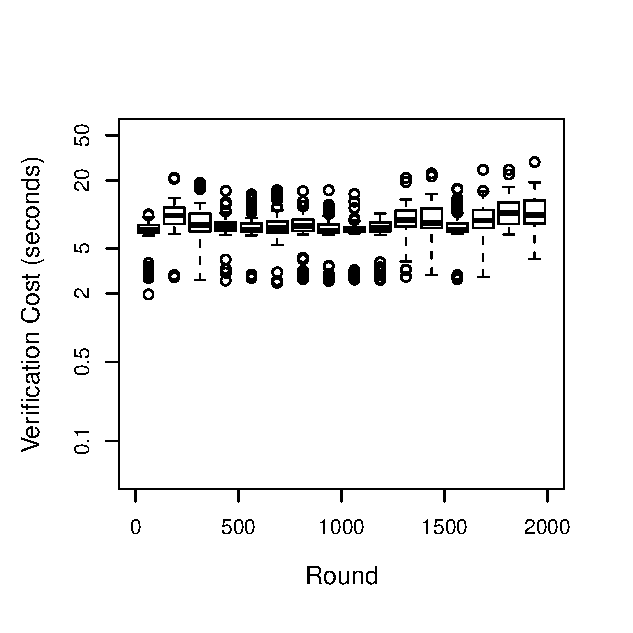
\epsfig{file=figures/tissec/xpilot_lazy_vanilla_time_box_uniform_scale.eps, width=\figurewidth}}
&
\subfigure[][{\parbox[t]{1.15in}{Cost per round (\lazy) with \xpilot-specific optimizations}}]{
	\label{fig:xpilottime:lazyopt}
	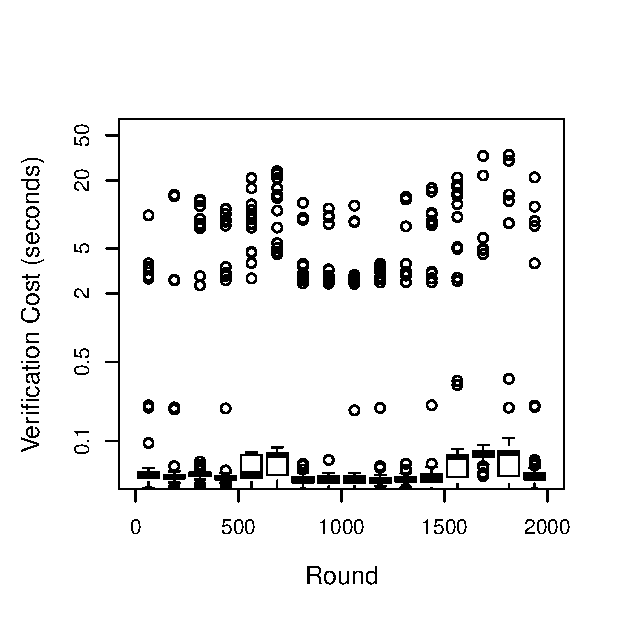
\epsfig{file=figures/tissec/xpilot_lazy_time_box_uniform_scale.eps, width=\figurewidth}}
&
\subfigure[][{\parbox[t]{1.15in}{Cost per round (\eager) with \xpilot-specific optimizations}}]{
	\label{fig:xpilottime:eageropt}
	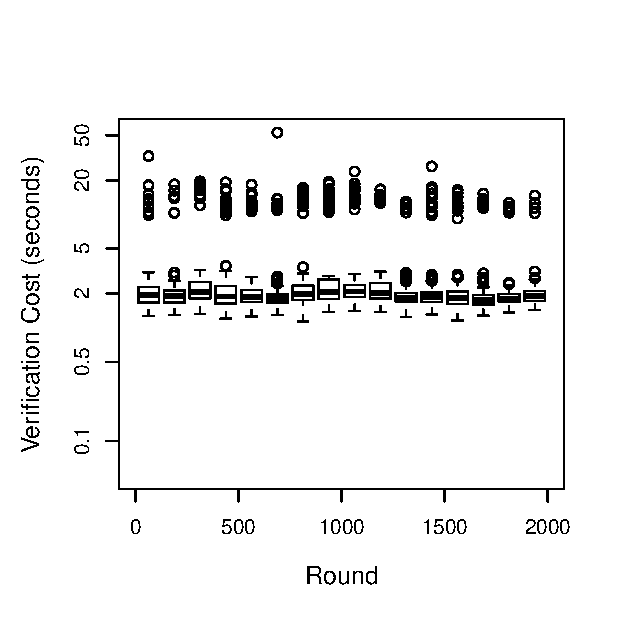
\epsfig{file=figures/tissec/xpilot_eager_time_box_uniform_scale.eps, width=\figurewidth}}
\end{tabular}
\caption{Verification cost per round while checking a 2,000-round
\xpilot game log \label{fig:xpilottime}}
\end{figure*}

By employing an \xpilot-specific optimization, we were able
to significantly improve verification performance.  After the trimming
described in \secref{ssec:scv:xpilot:mods}, the user input paths that we
included within our symbolic execution of the client each caused
another client-to-server message to be sent, and so the number of such
sends in a round indicates to the \verifier an upper bound on the
number of user inputs in that round.  As such, we could tune the
\verifier's symbolic execution to explore only paths through the
client where the number of invocations of the input-handling function
equals the number of client messages for this round in the log.  This
optimization yields the graph in Figure~\ref{fig:xpilottime:lazyopt}.
Notice that there are three distinct bands in the graph, corresponding
to how many times the input-handling function within the game client
was called.  The first band contains rounds which called the input
handler zero times and represents the majority (90.1\%) of the total
rounds.  These rounds were the quickest to process, with a mean cost
of 53.8ms and a standard deviation of 21.1ms.  The next-largest band
(5.1\%) contains rounds which called the input handler only once.
These rounds took longer to process, with a mean of 3.26s and a
standard deviation of 1.05s.  The final band represents rounds with
more than one call to the input-handling function.  This band took the
longest to process (12.9s, on average), but it was also the smallest, 
representing only 4.1\% of all rounds.

\subsection{Verification with \Eager \PathsegCons}
\label{ssec:scv:xpilot:eager}

In this section we discuss verification of \xpilot using \eager
constraint generation.  Recall that \eager \pathsegcons are
precomputed from the sanctioned client software without knowledge of
the messages the client will process in any given loop iteration.
However, we found this approach to require moderate manual tuning
to be practical, as we describe below.

\subsubsection{Manual Tuning}
\label{sssec:xpilot:eager:tuning}

A direct application of our method for generating \eager
\pathsegcons for the \xpilot client loop would replace the user key
press with symbolic input and any incoming server message with a
symbolic buffer and then use \klee to symbolically execute the
resulting client program.  Such a direct application, however,
encountered several difficulties.  In this section we describe the
main difficulties we encountered in this direct approach and the
primary adaptations that we made in order to apply it to the \xpilot
client.  These adaptations highlight an important lesson: the \eager
technique, while largely automatic, can require some manual tuning to
be practical.  Because our technique is targeted toward game
developers, we believe that allowing for such manual tuning is
appropriate.

\subsubsection{Frame processing}
In \xpilot, messages from the server to the client describing the
current game state are called {\em frames}.  Each frame is formed of a
chain of game {\em packets} (not to be confused with network packets).
The first and last packets in a frame are always special
start-of-frame and end-of-frame packets, called \pktstart and \pktend.
Figure~\ref{fig:xpframe} shows an \xpilot frame, containing a packet
of type \pktfuel and potentially others (indicated by ``$\ldots$'').
Packets are encoded as a single header byte followed by a packet data
section that can carry anything from a single byte to an
arbitrary-length string, depending on the packet type.  Frames may
contain multiple packet types and multiple instances of the same
packet type.

%\begin{wrapfigure}{r}{0.3\textwidth}
\begin{figure}[t]
  \centering
  \begin{tabular}{|c|}
    \hline
    \pktstart header \\[10pt] \hline \pktstart data \\ $\vdots$\\[10pt]
    \hline\hline
    \pktfuel header \\[10pt] \hline \pktfuel data \\$\vdots$\\[10pt]
    \hline\hline
    $\ldots$ \\[10pt]
    \hline\hline
    \pktend header \\[10pt] \hline \pktend data \\$\vdots$\\[10pt]
    \hline
  \end{tabular}
  \caption{\xpilot frame layout}
  \label{fig:xpframe}
\end{figure}
%\end{wrapfigure}

Consider the client's frame-processing algorithm.  Given a frame, it
first reads the packet header (i.e., the first byte), then calls the
handler for that packet, which processes the packet and advances the
frame pointer so that the new ``first byte'' is the packet header of
the next packet in the frame.  This continues until the packet handler
for \pktend is called, the return of which signifies the end of the
frame handling.  Therefore, given a completely symbolic buffer
representing the frame, our symbolic execution would need to walk the
client code for {\em each possible sequence} of packets in a frame, up
to the maximum frame size.  But \xpilot has dozens of packet types,
some of which include a very small amount data.  As evidence of the
infeasibility of such an approach, consider the following (very
conservative) lower bound on the number of packet sequences: There are
at least 10 types of packets that we considered whose total size is at
most 5 bytes.  The maximum size for a server-to-client frame in
\xpilot is 4,096 bytes, which means there is room for over 800 of
these packets.  That gives {\em at least} $10^{800}$ possible packet
sequences that symbolic execution would traverse to generate
constraints, which is obviously infeasible.

To make \eager constraint generation feasible, then, we adapt our
approach to generate \pathsegcons by starting and stopping symbolic
execution at multiple points within the loop, as opposed to just the
beginning and end.  In particular, we apply symbolic
execution to the frame-processing and user input-processing portions
of the loop separately, to obtain {\em \inputcons} and {\em
  \framecons}, which in turn the \verifier pieces together {\em during
  verification} to construct the \pathsegcons.  Moreover, the
\verifier can construct the \framecons on the basis of the particular
frame the server sent to the client.  It does so dynamically from
\packetcons that characterize how the client should process each
packet in the particular frame.  For example, if the only
packet types were \pktstart, \pktfuel, \pkttimeleft, and \pktend, the
\packetcons representing the processing of a single packet would be
\[\begin{array}{l}
( \packettype = \pktstart ) \wedge (\constraintsfor{\pktstart}) \\
( \packettype = \pktfuel ) \wedge (\constraintsfor{\pktfuel}) \\
( \packettype = \pkttimeleft ) \wedge (\constraintsfor{\pkttimeleft}) \\
( \packettype = \pktend ) \wedge (\constraintsfor{\pktend})
\end{array}\]
where \packettype is a variable for the packet type and
\constraintsfor{\pktstart} represents the additional constraints that
would result from symbolic execution of the packet handler for
\pktstart.  With this new model of packet processing, the \verifier
can build a \framecon to represent any given frame from the logs.  In
this way, when the \verifier checks the behavior of a given client, it
does so armed with the frames the server sent to the client, the
messages the server
received from the client, and the \framecons that characterize the
client's processing of each frame, which the \verifier constructs from
the \packetcons.

\subsubsection{Packet processing} Certain individual packet types present
their own tractability challenges as well.  For example, the payload
for a certain packet begins with a 32-bit mask followed by one byte
for each bit in the mask that is equal to 1.  The client then stores
these remaining bytes in a 32-byte array at the offsets determined by
the mask (setting any bytes not included in the message to 0).  In the
packet handler, the \xpilot client code must sample the value of each
bit in the mask in turn.  Since the payload (and thus the mask) is
symbolic, each of these conditionals results in a fork of two separate
paths (for the two possible values of the bit in question).  Our
symbolic execution of this packet handler, then, would produce over 4
billion \pathsegcons, which is again infeasible.  We could have
changed the \xpilot protocol to avoid using the mask, sending 32 bytes
each time, but doing so would increase network bandwidth needlessly.
Instead, we note that the result of this packet handler is that the
destination array is set according to the mask and the rules of the
protocol.  We thus added a simple rule to the \verifier that, when
processing this type of packet, generates a constraint defining the
value of the destination array directly, as the packet handler would
have.  Then, when symbolically executing the packet handlers, we can
simply skip this packet.

To avoid similar modifications to the extent possible, we pruned the
packets the \verifier considers during verification to only those that
are necessary.  That is, there are several packet types that will not
alter the permissible behaviors of the client as could be witnessed by
the server, and so we ignored them when applying our technique.  Most
of these packet types represent purely graphical information.  For
example, a packet of type \pktitem simply reports to the client that a
game item of a given type (e.g., a power-up or a new weapon) is
floating nearby at the given coordinates.  This information allows the
client to draw the item on the screen, but it does not affect the
valid client behaviors as observable by the \verifier.\footnote{In
  particular, whether the client processes this packet is irrelevant
  to determining whether the client can pick up the game item
  described in the packet.  Whether the client obtains the item is
  unilaterally determined {\em by the server} based on it computing
  the client's location using the low-level client events it receives
  --- an example of how nearly all control is stripped from clients in
  today's games, owing to how they cannot be trusted.}

\subsubsection{User input}
The first part of the client input loop checks for and handles input
from the player.  Gathering \inputcons is fairly straightforward, with
the exception that \xpilot allows players to do an extensive amount of
keyboard mapping, including configurations in which multiple keys are
bound to the same function, for example.  We simplified the generation
of constraints by focusing on the user actions themselves rather than
the physical key presses that caused them.  That is, while generating
constraints within the user-input portion of \xpilot, we begin
symbolic execution {\em after} the client code looks up the in-game
action bound to the specific physical key pressed, but {\em before}
the client code processes that action.  For example, if a user has
bound the action \keyfireshot to the key `{\tt a}', our analysis would focus
on the effects of the action \keyfireshot, ignoring the actual key to
which it is bound.  However, as with other client configuration
options, the keyboard mapping could easily be sent to the server as a
requirement of joining the game, invoking a small, one-time bandwidth
cost that would allow the \verifier to check the physical key
configuration.

\subsubsection{\Eager Verification Performance}
\label{sssec:xpilot:eager:eval}

We ran our \eager client verifier on the same 2,000-round \xpilot game
log and on the same computer used in \secref{ssec:scv:xpilot:lazy}.
Figure~\ref{fig:xpilottime:eageropt} describes the per-round
validation cost (in seconds) using a box-and-whiskers plot.  As in
Figure~\ref{fig:xpilottime:lazyopt}, we employed here an
\xpilot-specific optimization by observing that the number of client
messages in a round bounds the number of user inputs in that round.
As such, in piecing together \pathsegcons, the \verifier includes a
number of copies of \inputcons (see \secref{sssec:xpilot:eager:tuning})
equal to the client sends in that round.  Similar to
Figure~\ref{fig:xpilottime:lazyopt},
Figure~\ref{fig:xpilottime:eageropt} exhibits three bands (the third
comprising a few large values), corresponding to different numbers of
copies.  The large percentage of rounds contained no user inputs and
were the quickest to process, with a mean cost of 1.64s and a standard
deviation of 0.232s.  The second band of rounds --- those with a
single user input --- took longer to process, with a mean of 11.3s and
a standard deviation of 1.68s.  Remaining rounds contained multiple
user inputs and took the longest to process (34.2s, on average), but
recall that they were by far the least frequent.  The \verifier's
memory usage remained below 100MB throughout these verification runs.

Comparing
Figures~\ref{fig:xpilottime:lazyopt} and~\ref{fig:xpilottime:eageropt},
the times for the \eager approach are much slower than those
for the \lazy approach, when applied to \xpilot.  This performance
loss is due to the fact that a large portion of the \xpilot client
code is dedicated to handling server messages.  And while the
\verifier in the \eager case has preprocessed this portion of the
code, the resulting \pathsegcons are much more complex than in the
\lazy approach, where the \verifier knows the exact values of the
server messages when generating \pathsegcons.  This complexity results
in constraint solving in the \eager case
(line~\ref{fig:trackConstraints:isSat} of
Figure~\ref{fig:trackConstraints}) being more expensive.

It is also important to recall that \lazy and \eager are not
interchangeable, at least in terms of game developer effort.  As
discussed in \secref{sssec:xpilot:eager:tuning}, achieving feasible
generation of \eager \pathsegcons required substantial additional
manual tuning, and consequently greater opportunity for programmer
error.  As such, it appears that the \eager approach is inferior to
the \lazy approach for \xpilot.  Another comparison between the two
approaches, with differing results, will be given in
\secref{sec:scv:capman}.

\section{Case Study: \capman}
\label{sec:scv:capman}

Our client verification technique challenges the current game-design
philosophy by allowing servers to relinquish authoritative state to
clients while retaining the ability to validate client behavior and
thus detect cheating.  As a way of demonstrating this notion, we have
written a game called \capman that is based on the game \pacman.  In
some ways \capman is easier to validate than \xpilot was --- it
represents a considerably smaller code base (roughly 1,000 lines
of C code) and state size.

That said, \capman is interesting as a case study for three reasons.
First, whereas \xpilot was written with virtually no authoritative
client state, we will see that \capman is intentionally rife with it,
providing a more interesting challenge for our technique because it is
so much more vulnerable to invalid messages.  Second, the size of its
code base allows us to conduct a more direct comparison between \lazy
and \eager verification.  Third, \capman differs from \xpilot in that
the set of possible user inputs per round is substantially larger than
the set of paths through the client's event loop.  That is, in
\xpilot, there is nearly a one-to-one correspondence between user
inputs and paths through the client event loop, which dampens the
improvement that our technique offers over, e.g., the \verifier simply
running the client on all possible inputs in each round.  \capman
demonstrates the scalability of our technique to many possible user
inputs when this is not the case, thereby separating our technique
from other such possible approaches.

\subsection{The Game}

\capman is a \pacman-like game in which a player controls an avatar
that is allowed to move through a discrete, two-dimensional map with
the aim of consuming all remaining ``food'' items before being caught
by the various enemies (who are also navigating the map).  Each map
location is either an impenetrable wall or an open space, and the open
spaces can contain an avatar, an enemy, pieces of food, a power-up, or
nothing at all.  When a player reaches a map location that contains
food or a power-up, he automatically consumes it.  Upon consuming a
power-up, the player enters a temporary ``power-up mode,'' during
which his pursuers reverse course --- trying to escape rather than
pursue him --- and he is able to consume (and temporarily displace)
them if he can catch them.  In addition to these features (which were
present in \pacman as well), we have added a new feature to \capman to
invite further abuse and create more uncertainty at the server: A
player may set a bomb (at his current location), which will then
detonate a number rounds in the future selected by the user from a
predefined range (in our implementation, between 3 and 15
rounds).\footnote{In our preliminary work~\cite{bethea10:games}, a
  bomb detonated in a fixed number of rounds.  We changed the game to
  accommodate a user-selected number of rounds to bomb detonation in
  order to demonstrate the ability of our technique to scale to a
  larger number of possible user inputs.}  When it detonates, it kills
any enemies (or the player himself) within a certain radius on the
map.  Players are not allowed to set a new bomb until their previous
bomb has detonated.

\capman uses a client-server architecture, which we designed
specifically to go against current game-development best practices:
i.e., it is the {\em server}, not the client, which has a minimum of
authoritative state.  The client tracks his own map position,
power-up-mode time remaining, and bomb-placement details.
Specifically, at every round, the client sends a message to the server
indicating its current map position and remaining time in power-up
mode.  It also sends the position of a bomb explosion, if there was
one during that round.  Note that the client never informs the server
when it decides to {\em set} a bomb.  It merely announces when and
where detonation has occurred.  The server, in contrast, sends the
client the updated positions of his enemies --- this being the only
game state for which the server has the authoritative copy.

The design of \capman leaves it intentionally vulnerable to a host of
invalid-message attacks.  For example, although valid game clients
allow only contiguous paths through the map, a cheating player can
arbitrarily adjust his coordinates, ignoring the rules of the game ---
a cheat known in game-security parlance as ``telehacking.''  He might
also put himself into power-up mode at will, without bothering to
actually consume a power-up.  Finally, there is no check at the server
to see whether or not a player is lying about a bomb placement by, for
example, announcing an explosion at coordinates that he had not
actually occupied within the past 15 rounds.  In fact, the \capman
server contains no information about (or manual checks regarding) the
internal logic of the game client.

In order to detect cheating in \capman, we apply our technique in both
its \lazy and \eager variations.  Due to \capman's smaller size and
simpler code structure, we can generate \pathsegcons over an entire
iteration of the main loop in each case, without the need to
compartmentalize the code and adopt significant trimming measures as
we did for \xpilot.

\subsection{Evaluation}

Using our technique, we are able to detect invalid-command cheats of
all the types listed above.  Below we present the results of
client-validity checks on a game log consisting of 2,000 rounds (about
6-7 minutes of game-play time), during which the player moved around the
map randomly, performing (legal) bomb placements at random intervals.

\begin{figure*}[t]
\hspace{-5pt}
\begin{tabular}{@{\extracolsep{-1.25em}}ccc}
\subfigure[][{\parbox[t]{1.1in}{Cost per round (\lazy)}}]{
	\label{fig:capmantimes:lazy}
	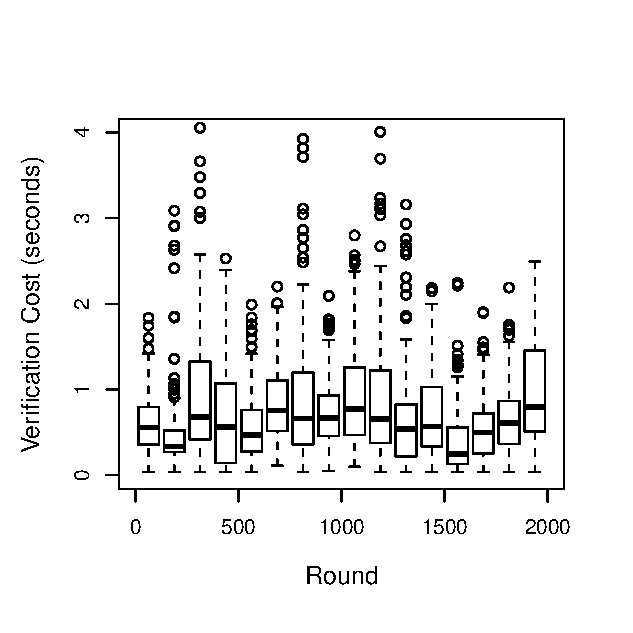
\epsfig{file=figures/tissec/capman_lazy_time_box.eps, width=\figurewidth}}
&
\subfigure[][{\parbox[t]{1.15in}{Cost per round (\eager)}}]{
	\label{fig:capmantimes:eager}
	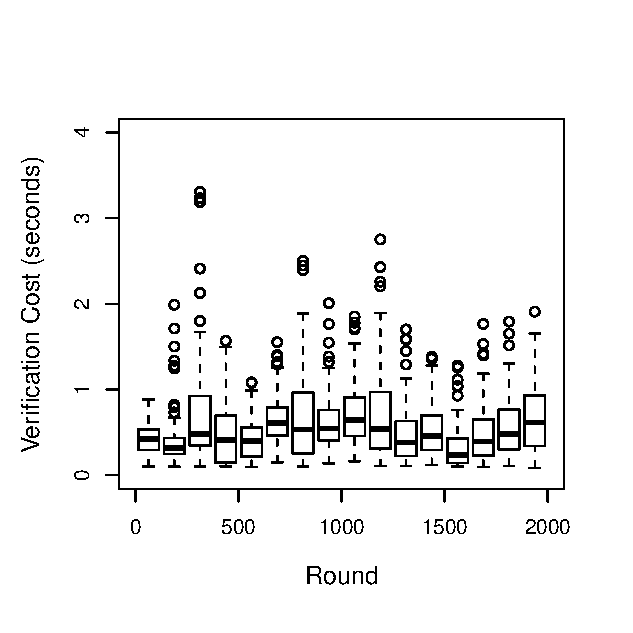
\epsfig{file=figures/tissec/capman_eager_time_box.eps, width=\figurewidth}}
&
\subfigure[][{\parbox[t]{1.5in}{Satisfiable \execpathcons per round (\eager)}}]{
	\label{fig:capmanchainsplot}
	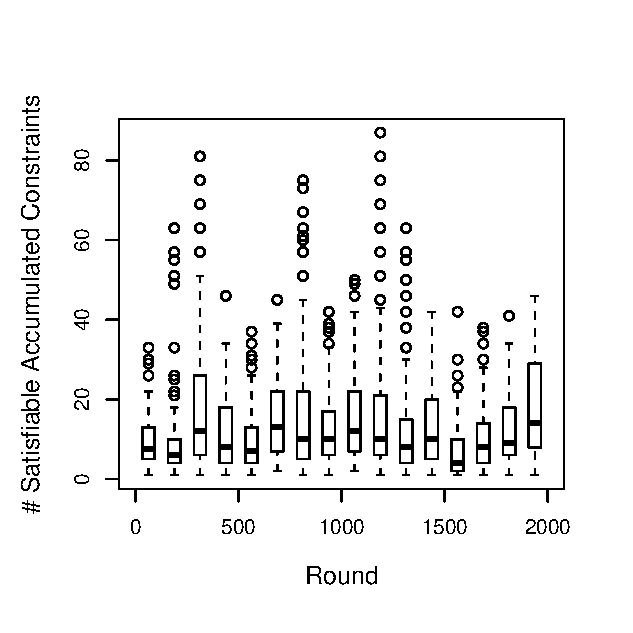
\epsfig{file=figures/tissec/capman_eager_chains_box.eps, width=\figurewidth}}
\end{tabular}
\caption{Verifying a 2,000-round \capman game log}
\label{fig:capmantimes}
\end{figure*}

Figure~\ref{fig:capmantimes} shows that the verification costs for
\capman were consistently small, with a mean and standard deviation of
752ms and 645ms for verification via \lazy \pathsegcons
(Figure~\ref{fig:capmantimes:lazy}) and a mean and standard deviation
of 310ms and 193ms for verification using \eager \pathsegcons
(Figure~\ref{fig:capmantimes:eager}).  The \lazy method was (on
average) roughly 2.5 times slower than the \eager method, owing to the
overhead of symbolic execution to compute \pathsegcons for each round
individually during verification.  The \verifier's memory usage
remained below 100MB throughout verification of both types.  While in
the \xpilot case study, \eager verification required significantly
greater development effort (see \secref{sssec:xpilot:eager:tuning}),
this additional effort was unnecessary with \capman due to its
relative simplicity.

Figure~\ref{fig:capmanchainsplot} shows the number of satisfiable
\execpathcons during \eager verification, which did not trend upward
during the run.  In \lazy verification, the number of satisfiable
\execpathcons was virtually identical.  (Variations in our pruning
implementations caused less than $1\%$ of the rounds to differ, and
then by at most 12 \execpathcons.) In the case of \xpilot, the number
of satisfiable \execpathcons was always $1$, but in \capman there were
often multiple \execpathcons that remained satisfiable at any given
round.  This increase resulted primarily from state the \capman client
maintains but does not immediately report to the server (e.g., whether
a bomb has been set, and with what detonation timer).  The
relationship between this hidden state and the number of satisfiable
\execpathcons is an important one.  Consider the verification of a
\capman game that is currently in round $\roundidx$, with no bomb
placements in the last 15 rounds (unbeknownst to the \verifier).  The
\verifier must maintain \execpathcons that reflect possible bomb
placements at each of rounds $\roundidx-14$ through $\roundidx$.  Upon
encountering $\clientMsg_{\roundidx+1}$ with an announcement of a bomb
explosion, the \verifier can discard not only all current
\execpathcons which do {\em not} include a bomb placement in any of
rounds $\roundidx-14$ through $\roundidx-2$, but also those
\execpathcons which {\em do} include bomb placements in rounds
$\roundidx-1$ through $\roundidx+1$, because players can only have one
pending bomb at a time.  This rule was not manually configured into
the \verifier; it was inferred automatically from the client code.

\section{Case Study: \tetrinet}
\label{sec:scv:bandwidth}

As discussed earlier, our verification technique
presents opportunities to reduce the bandwidth consumed by an online
game, since it allows the client's management of state to be verified
with less-than-complete information.
In our third case study, we used a pre-existing game called \tetrinet
in order to explore simple bandwidth-savings measures and their impact
on client verification performance.

\subsection{The Game}
\tetrinet is a multiplayer clone of the classic puzzle game \tetris.
It was originally developed in 1997 but remains popular and has been
reimplemented on many different platforms.  In the game, random
\textit{tetrominoes}, which are geometric shapes consisting of four
connected blocks, automatically advance down each player's playing
field, one at a time.  As each does, the player can rotate it into
four possible orientations or slide it horizontally left or right.
The objective of the game is to arrange tetrominoes so that, as they
land, they create gapless horizontal rows of blocks on the playing
field.  When such a gapless row is created, it is cleared, each row of
blocks above it falls down one row, and --- in the primary multiplayer
departure from \tetris{} --- a line with gaps is added to the bottom
of the other players' fields.  A player loses when there is no room
for an additional tetromino to enter her playing field.  \tetrinet is
implemented in C and has a client-server architecture similar to
\capman and \xpilot.  The server does virtually no checking on client
messages and so is vulnerable to cheats; e.g., a client could indicate
it cleared a row that has gaps or placed a new tetromino in a spot
that the client should not have allowed it to reach.

Enabling the use of our verification tool with \tetrinet required some
consideration of how the user input operates. A tetromino in play
automatically moves down one row every $0.5$~seconds, and when the
piece can move no further, the position is fixed and a new random
piece starts falling from the top of the game screen. The placement of
the tetromino in a permanent resting point defines the end of single
round of gameplay, at which time the \tetrinetHorizontal and
\tetrinetVertical coordinates and the rotation \tetrinetOrientation
are sent to the server. Until the end of the round, though, the player
can move the piece horizontally or rotate it as many times as she
wishes. So, even though there is a finite number of final fixed
positions for a game piece in a given round, there are theoretically
an infinite number of possible inputs sequences that could lead to
each valid final position. To minimize the number of input sequences
that must be explored symbolically, we considered a restricted version
of gameplay where the gameboard must be empty above each tetrimino at
the time of its placement, and so three rotations and six horizontal
moves sufficed to reach any such placement on the 12-column gameboard.

\subsection{Evaluation}
To demonstrate bandwidth reduction in \tetrinet using our verification
technique, we simply reduced the information in the client-to-server
messages. \tetrinet was modified so that only every
\tetrinetUnabridgedFreq rounds was the complete tuple
$(\tetrinetHorizontal, \tetrinetVertical, \tetrinetOrientation)$ sent
to the server (an ``unabridged message'').  In other rounds, the
client sent a partial tuple, omitting \tetrinetHorizontal,
\tetrinetVertical, or \tetrinetOrientation or both \tetrinetVertical
and \tetrinetOrientation.  Figure~\ref{fig:tetrinettimes} shows the
tradeoff between the bandwidth reductions accomplished and the costs
of verifying client behavior using the \lazy client verifier, where
the bandwidth reductions were calculated assuming \tetrinetHorizontal,
\tetrinetVertical and \tetrinetOrientation are sent in four, five, and
two bits, respectively.  (The actual \tetrinet implementation is not
engineered for bandwidth reduction and so uses payload space more
wastefully.)  These graphs each represent five random play sessions of
100 rounds each and the same five play sessions were used for each of
the four experiments.  Note that $\tetrinetUnabridgedFreq=1$ is
equivalent to verification of an unmodified game client. In the
experiment where \tetrinetVertical is omitted, the verification cost
does not increase because there is no ambiguity as to
\tetrinetVertical's value when \tetrinetHorizontal and
\tetrinetOrientation are provided. During these verification runs,
the \verifier's memory usage remained below 512MB.

\begin{figure}[t]
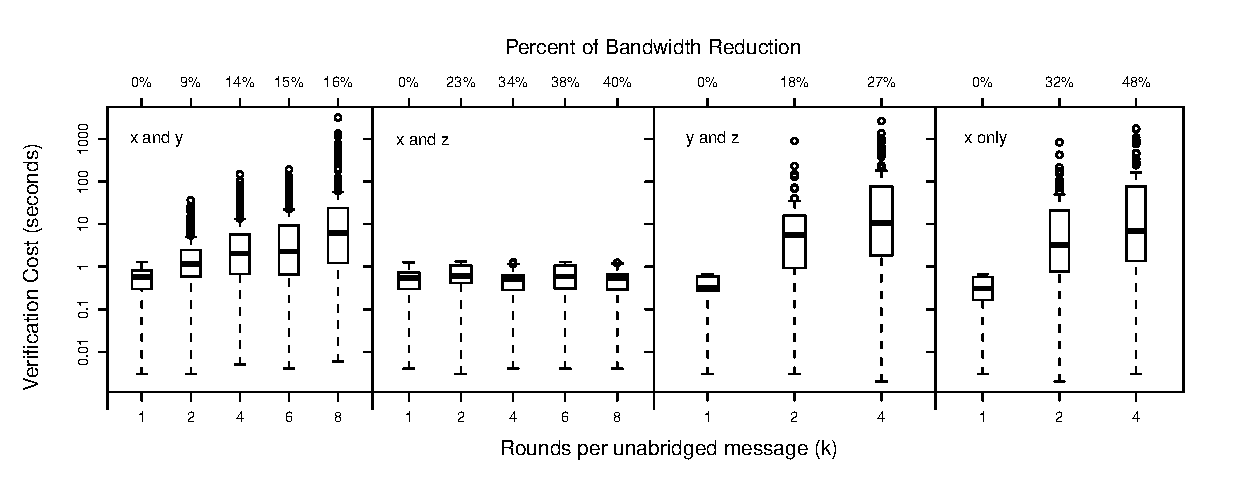
\epsfig{file=figures/tissec/tetrinet_time_vs_bandwidth_grid.eps, width=\textwidth}
\caption{Verification of 100-round \tetrinet logs under different
configurations of client-to-server message content.}
\label{fig:tetrinettimes}
\end{figure}

\section{Verification with message loss}
\label{sec:scv:message-loss}

Games today must be built to tolerate a range of networking
conditions, including occasional message loss.  While there are
standard approaches to recovering lost messages, such as message
retransmission at the transport level (i.e., using TCP) or at the
application level, retransmission is avoided in some games for two
reasons.  First, the importance of some messages diminishes quickly,
and so by the time the message would be retransmitted, the utility of
doing so is lost.  Second, retransmission can introduce overheads that
high-performance games cannot tolerate.


Lost server-to-client messages pose little difficulty to our client
verification technique; all the \verifier requires is to know what
server-to-client messages the client processed and when, which can be
communicated from the client efficiently (e.g., see
\secref{app:acks}).  Lost client-to-server messages pose more
difficulty, however.  Intuitively, our technique can handle client
message loss by instantiating the constraint \msgConstraint for a
missing round-\roundidx message $\clientMsg_{\roundidx}$ to simply
$\msgConstraint = ``\mathrm{true}"$ in
Figure~\ref{fig:trackConstraints}.  However, this has two negative
consequences.

First, from the server's (and \verifier's) perspective, it is
impossible to distinguish a lost message from one the client only
pretended to send.  This can be used by a cheating client to gain
latitude in terms of the behaviors that the \verifier will consider
legitimate.  For example, whenever a power-up appears on the game map,
an altered game client could collect it by reporting its player's
position at the power-up's location.  So as to not be caught by the
\verifier, the client could alter its state to reflect having sent
messages that would have been induced by the player actually moving to
that location, even though these messages were never sent and so, from
the server's perspective, were lost. Because it is possible for a
valid client on a poor network connection to generate
indistinguishable behavior, this cheat is not in the class that our
\verifier detects. Nevertheless, as discussed in
\chref{ch:background},
our techniques are compatible with existing methods that address this
type of cheat.

Another consequence of message loss is that the performance of
verification can be severely impacted by it.  The performance results
in \secref{sec:scv:xpilot}--\ref{sec:scv:capman} did not reflect the loss of
any client messages; instead, the game logs that we validated included
all messages that the client sent.  However, in practice message loss
causes the \execpathcons $\execPathConstraints_{\roundidx}$
to grow dramatically, since {\em any} path through the client that
causes a message to be sent is deemed possible in round \roundidx.  As
a result, in experimenting with message loss in \xpilot, we found that
in the face of lost messages, the performance of our technique decays
very substantially.

As such, we propose a lightweight scheme to enable our technique to
retain its performance in the face of (limited) message loss.  Rather
than retransmitting messages, our technique communicates a small
amount of additional information per client-to-server message to
enable the \verifier to prune \execpathcons effectively in the face of
message loss.  Intuitively, the client remembers the path through its
event loop that it traverses in round \roundidx and then conveys
evidence of this to the server over the next several messages.  The
server records this evidence for the \verifier, which uses it to prune
\pathsegcons considered for round \roundidx.

There are several ways to instantiate this intuition within our
framework.  Here we describe one implementation that works well in
\xpilot.  In this implementation, the ``evidence'' that the client
conveys to the server for the path it traversed in round
\roundidx is a hash of the fields of the message it sent in round
\roundidx that are a function of (only) the path traversed.
Rather than send the entire hash in a subsequent message, however, the
client ``trickles'' this hash value to the server, e.g., one bit per
message, so that subsequent message losses still enable the server to
collect a number of hash bits for each round.  After the client's
messages are recorded at the server, the \verifier collects these bits
and uses them to prune the \pathsegcons considered at each step of
verification where it is missing a message.

We have prototyped this approach in the context of \lazy verification,
in order to validate the ability of the \xpilot \verifier to retain
its performance in the face of message losses.  (\capman and \tetrinet
use TCP and so do not face message-loss issues.)  The hash we use is a
\hashsize-bit BSD \texttt{sum}, and the \bitidx-th bit of the
round-\roundidx message hash is carried on the round
$\roundidx+\bitidx$ message ($1 \le \bitidx \le \hashsize$).  As such,
each message carries an extra \hashsize bits composed of bits from the
previous \hashsize client-to-server messages.

%\begin{wrapfigure}{r}{0.35\textwidth}
\begin{figure}[t]
\centering
%\vspace{-0.2in}
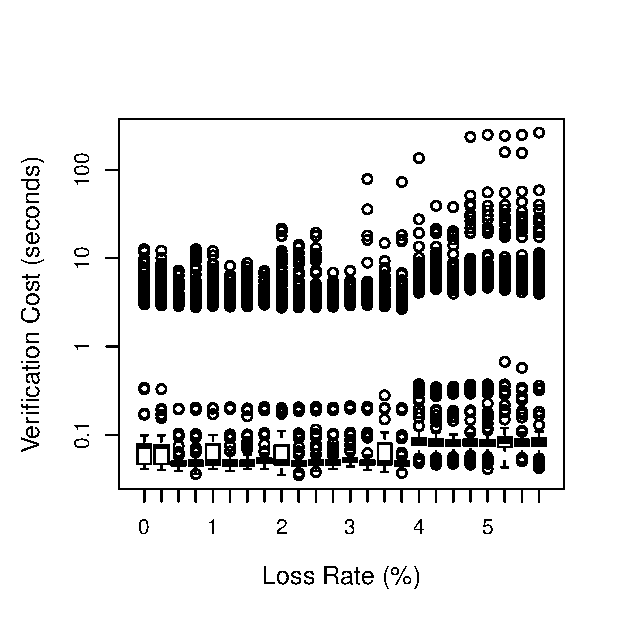
\epsfig{file=figures/tissec/xpilot_lazy_lossrates_box.eps, width=\figurewidth}
%\vspace{-0.1in}
\caption{Verification (\lazy) of 2000-round \xpilot log with loss of
client-to-server messages at the rate indicated on horizontal axis.}
\label{fig:random_loss} 
%\vspace{-0.1in}
%\end{wrapfigure}
\end{figure}

To show the effectiveness of this approach, we repeated the
\lazy verification of $2000$-round \xpilot game logs using \xpilot-specific
optimizations (c.f., Figure~\ref{fig:xpilottime:lazyopt}) but
introduced client-to-server message losses to show that our approach
tolerates them seamlessly.  We experimented with two types of message
loss.  In the first, each client-to-server message is lost with a
fixed probability.  Figure~\ref{fig:random_loss} shows
box-and-whiskers plots that illustrate the per-round verification
costs that resulted, as a function of this loss rate.  Note that a
message loss rate of 4\% earns a ``critical'' designation at a
real-time monitoring site like \url{www.internetpulse.net}.  As
Figure~\ref{fig:random_loss} shows our technique can easily handle
such a high loss rate.

A second type of loss with which we experimented is a burst loss,
i.e., the loss of a contiguous sequence of client-to-server messages.
Figure~\ref{fig:burst_loss} shows the verification costs per round in
five different message logs in which a burst loss of length $6$, $10$,
or $14$ client-to-server messages is introduced at a random point
between the $100$th and $150$th round.  As these graphs show, the
verification costs do tend to spike in the region where the burst loss
occurs, but the verification costs remain feasible and recover after
the burst to their original durations.  Only when the burst length
exceeds \hashsize (not shown) do the verification costs become and
remain too large to be practical.

%\clearpage
\begin{figure}[ht]
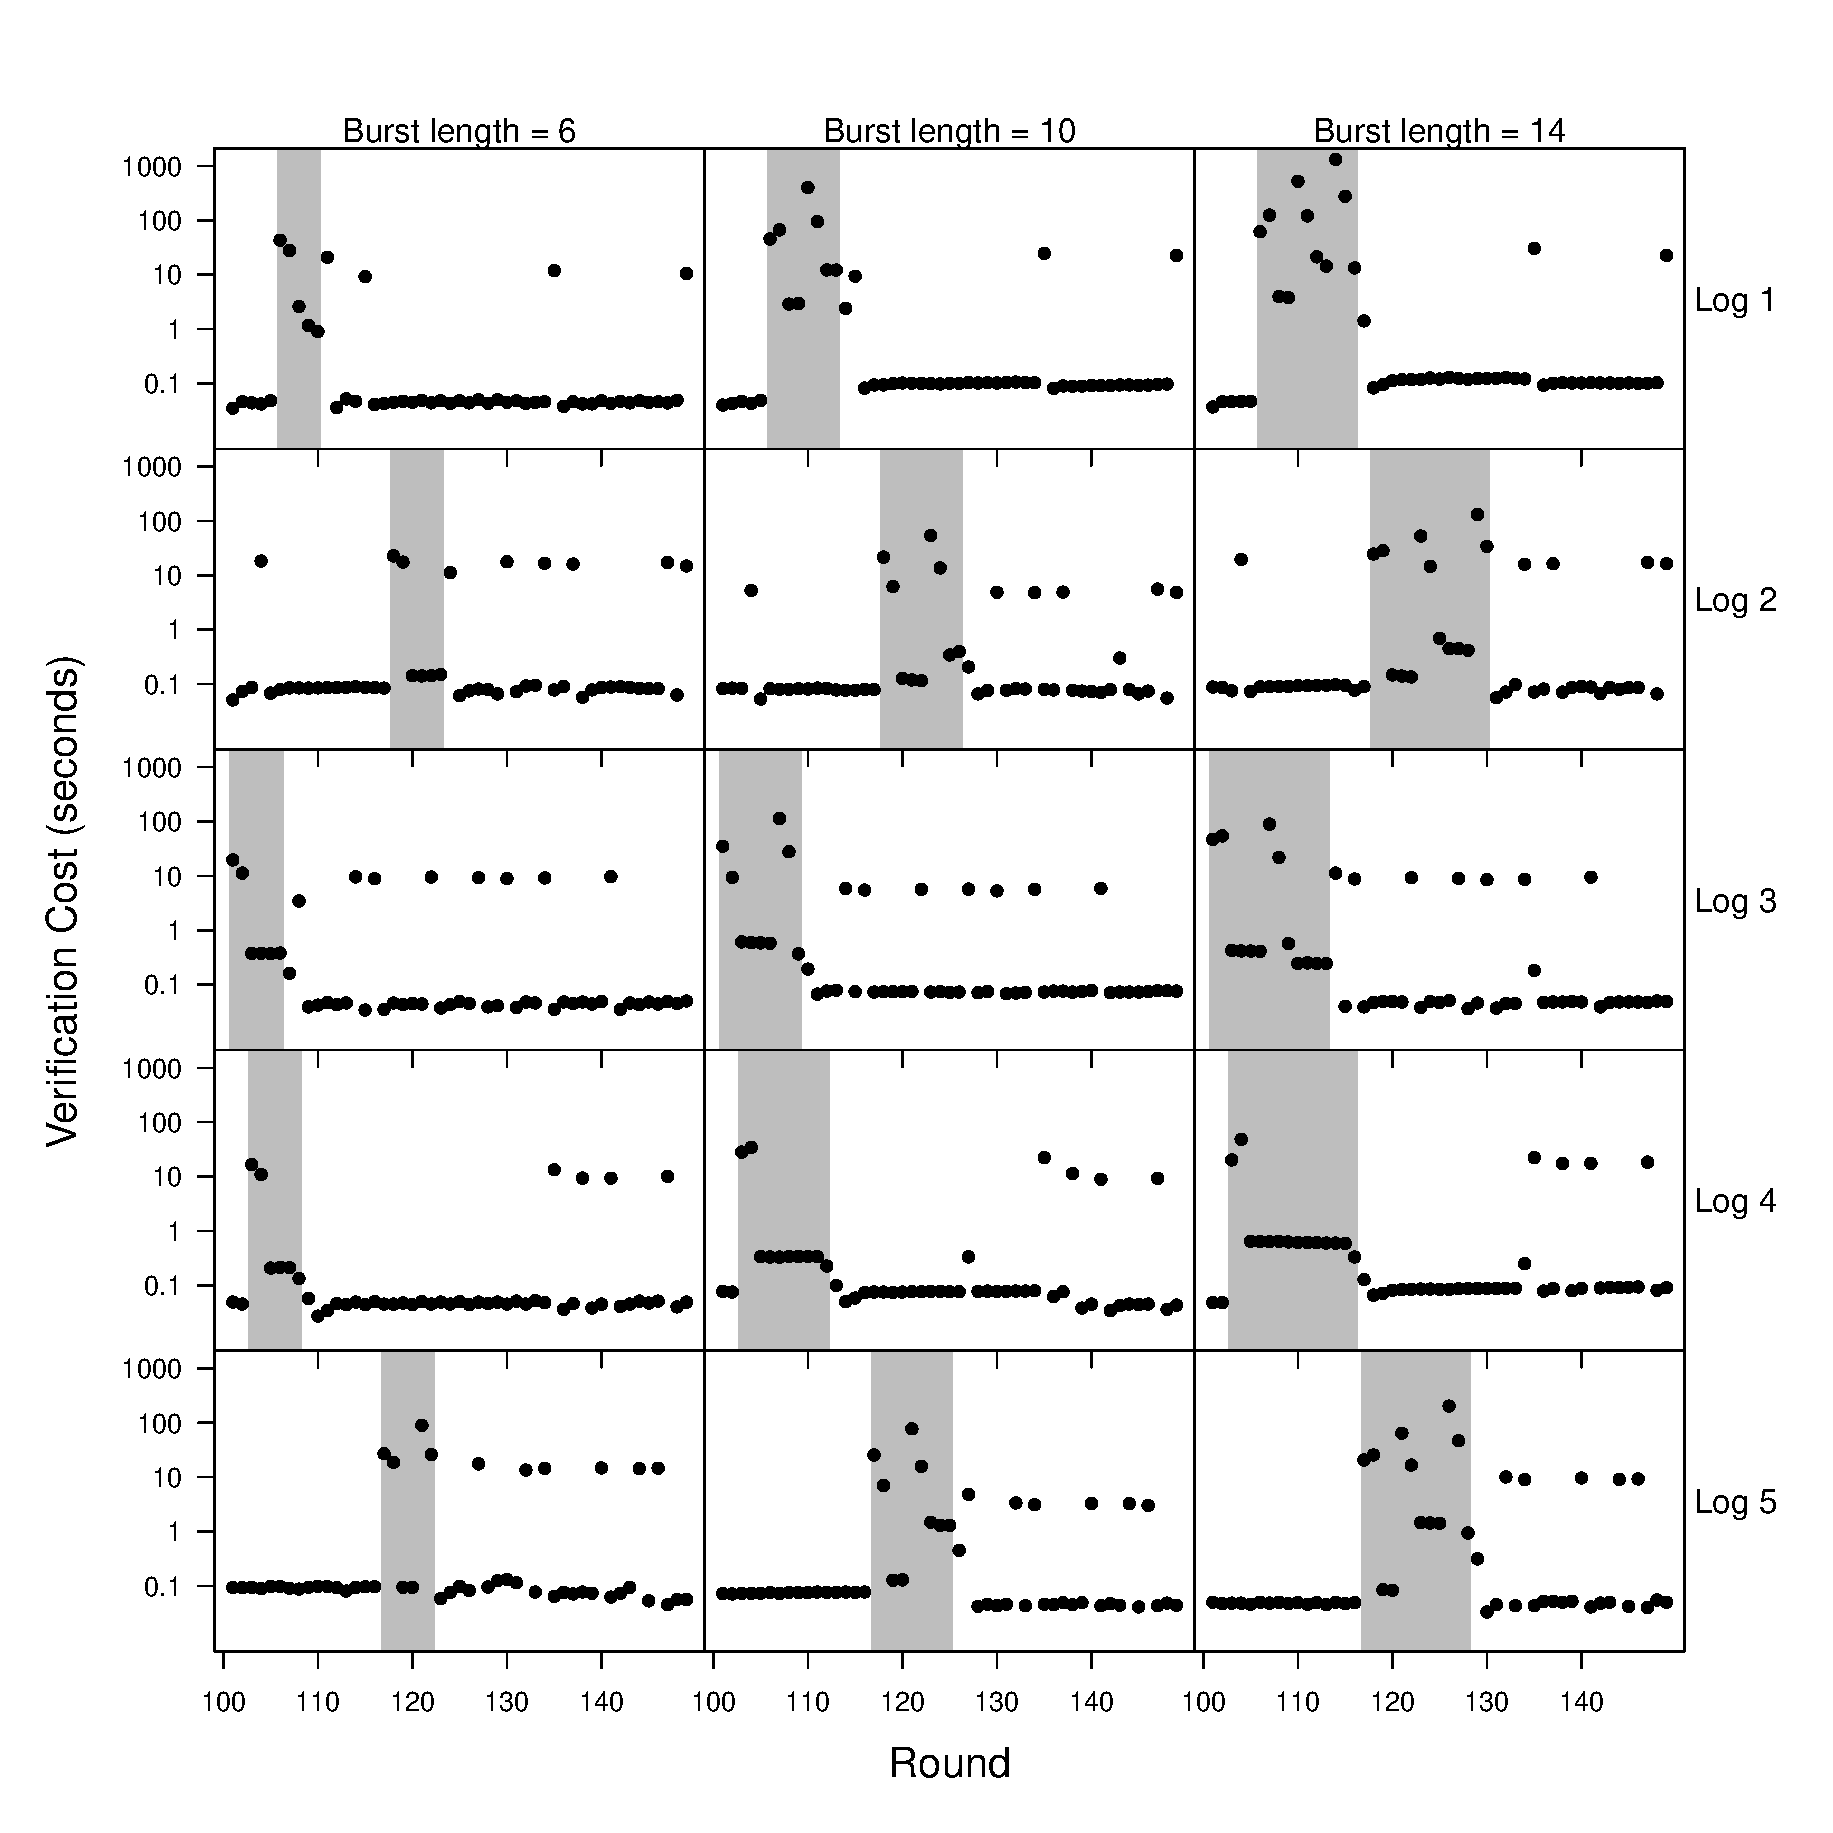
\epsfig{file=figures/tissec/xpilot_lazy_burstsize_grid.eps, width=\textwidth}
\caption{Verification (\lazy) of \xpilot logs with randomly induced
bursts of client-to-server message losses.  Shaded areas designate
rounds in which losses occurred.}
\label{fig:burst_loss}
\end{figure}
\clearpage

%\subsection*{Acknowledgements}
%
%We are deeply grateful to Cristian Cadar, Daniel Dunbar, and Dawson
%Engler for helpful discussions and for permitting us access to an
%early release of \klee.  Srinivas Krishnan, Alana Libonati, Andy White
%and the anonymous reviewers provided helpful comments on drafts of
%this paper.  This work was supported in part by NSF awards 0756998,
%0910483, and 1115948.

\section{Acknowledgement Scheme for \xpilot}
\label{app:acks}

As discussed in \secref{ssec:scv:xpilot:mods}, an efficient acknowledgement
scheme allows the server (and hence \verifier) knowledge of the order
(and loop iterations) in which the client processed server messages
and sent its own messages.  Below we describe one such scheme that is
optimized for messages that arrive at the client mostly in order.

In this scheme, the \xpilot client includes a sequence number \cToSNbr
on each message it sends to the server, and similarly the server
includes a sequence number \sToCNbr on each message it sends to the
client.  Each message from the server to a client also includes the
largest value of \cToSNbr received from that client.  In each client
message, the client includes \cToSAckd, the largest value of \cToSNbr
received in a server message so far; a sequence \lateMsgs{} of server
message sequence numbers; and a sequence \symbSeq{} of symbols that
encode events in the order they happened at the client.  The symbols
in \symbSeq{} can be any of the following.  Below, \sToCAckd is the
largest sequence number \sToCNbr received by the client before sending
message \cToSAckd, and similarly \loopAckd is the largest client loop iteration
completed at the client prior to it sending \cToSAckd.

\begin{itemize}
\item \symbLoop denotes a completed loop iteration.  The $\symbLoopCtr$-th
occurrence of \symbLoop in \symbSeq{} denotes the completion of loop
iteration $\loopAckd + \symbLoopCtr$.
\item \symbSent denotes the sending of a message to the server.  The
$\symbSentCtr$-th occurrence of \symbSent in \symbSeq{} denotes the
sending of client message $\cToSAckd+\symbSentCtr$.
\item \symbRcvd and \symbSkip denote receiving or skipping the
next server message in sequence.  The $\symbRorSCtr$-th occurrence of
\symbRcvd or \symbSkip in \symbSeq{} denotes receiving or skipping,
respectively, server message $\sToCAckd+\symbRorSCtr$.  Here, a
message a skipped if it has not arrived by the time a server message
with a larger sequence number arrives, and so a series of one or more
\symbSkip symbols is followed only by \symbRcvd in \symbSeq{}.
\item \symbLate denotes the late arrival of a message, i.e., the
arrival of a message that was previously skipped.  The
$\symbLateCtr$-th occurrence of \symbLate in \symbSeq{} denotes the
arrival of server message \lateMsgs{\symbLateCtr}.
\end{itemize}

As such, \lateMsgs{} contains a sequence number for each server
message that arrives after another with a larger sequence number, and
so \lateMsgs{} should be small.  \symbSeq{} may contain more elements,
but the symbols can be encoded efficiently, e.g., using Huffman
coding~\cite{huffman52:codes}, and in at most three bits per symbol in
the worst case.  Note that the server can determine \sToCAckd and
\loopAckd based on the previous messages received from the client.

\section{Summary}
\label{sec:scv:conclusion}

%The need to detect cheats has heavily influenced the design of online
%games.  Cheating has driven game developers to minimize or eliminate
%authoritative state from game clients.  These measures have direct
%impact on the game operator's bottom line, due to the inflated
%bandwidth costs that result and to the manual and heuristic (and hence
%ongoing) effort of programming server-side checks on client behaviors.

In this chapter, we described an approach to validate the server-visible
behavior of remote clients.  Our approach validates that client
behavior is a subset of the behaviors that would be witnessed from the
sanctioned client software, in light of the previous behaviors of the
client and the messages sent to that client.  Our technique exploits
a common structure in clients, namely a loop that accepts server
and user inputs, manages client state, and updates the server with
necessary information.  Our technique
applies symbolic execution to this loop to produce constraints that
describe its effects.  The server operator can then automatically check
the consistency of client updates with these constraints offline.  We
explored both \lazy and \eager approaches to constraint generation and
investigated the programmer effort each entails, as well as their
performance.

We demonstrated our technique in the context of online games with 
three case studies.
In the first, we applied our validation approach to \xpilot, an
existing open-source game.  We detailed the ways we adapted our
technique, in both the \lazy and \eager variants, to allow for
efficient constraint generation and server-side checking.  While this
effort demonstrated applying our approach to a real game, it was less
satisfying as a test for our technique, in that \xpilot was developed
in the mold of modern games --- with virtually no authoritative state
at the client.  We thus also applied our technique to a simple game of
our own design that illustrated the strengths of our technique more
clearly.  We then showed simple ways to leverage our technique to
reduce bandwidth consumption in a game called \tetrinet, and returned
to \xpilot to demonstrate a strategy for dealing with message loss.

%We believe that our technique can change how game developers address
%an important class of game cheats today, and in doing so opens up new
%avenues of game design that permit lower bandwidth utilization and
%better performance.


